\chapter{\MakeUppercase{Построение траектории движения схвата и определение начальных условий для уравнений кинематики}}
Зададим программную ориентацию схвата с помощью матрицы направляющих косинусов. Выберем координату в которую будет позиционироваться схват:
\begin{align*}
    T_d &=\begin{bmatrix}
    1 &  0 &  0 & x_d \\
    0 & -1 &  0 & y_d \\
    0 &  0 & -1 & z_d \\
    0 &  0 &  0 & 1
    \end{bmatrix}; \:
    x_d = 0; \:
    y_d = 0,4; \:
    z_d = 0 = const
\end{align*}

\noindent После чего составим минимизируемую функцию, добавим ограничения на углы и найдем величины обобщенных координат в начальной точке траектории. Выбор этой точки основан на значении минимума функции $ g(F) $:
$$ g(F) = g(T - T_d) $$
$$ g(F) = F_{00}^2 + F_{01}^2 + \hdots + F_{33}^2 $$

\noindent Чем меньше значение этой функции в точке тем более точно схват может позиционироваться в ней. Далее продолжаем исследовать плоскую подобласть $ D $, определим ее границы и выберем еще две точки траектории:

\begin{figure}[ht]
    \centering
    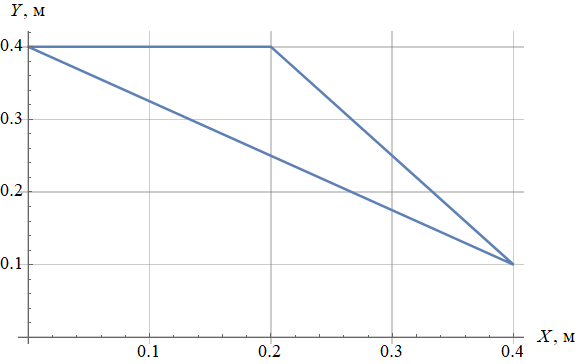
\includegraphics[scale=0.65]{plot_part3.png}
    \caption{Плоская подобласть $ D $ и траектория движения схвата}
\end{figure}
\newpage

\noindent Значения функций в трёх выбранных точках:
\begin{align*}
    F(x_d=0 , y_d=0,4 , z_d=0): g(F)=& 8,88*10^{-16} \\
    F(x_d=0,2 , y_d=0,4 , z_d=0): g(F)=& 4,44*10^{-15} \\
    F(x_d=0,4 , y_d=0,1 , z_d=0): g(F)=& 3,46*10^{-14}
\end{align*}




